\section{Application}
\label{sec:application}

\subsection{Data and model}
\label{sec:app-data}

At a roadside site the total oxidant $\mathrm{OX} = \mathrm{NO_2} +
\mathrm{O_3}$ is close to linear in the concentration of the nitrogen oxides
NOx \citep[Section~2.3]{Clapp-Jenkin-2001}: the intercept is the regional
background of oxidant, and the slope is the local contribution to it, which
\citet[Section~2.4]{Carslaw-Beevers-2005} use as an estimate of the fraction
of NOx emitted directly as $\mathrm{NO_2}$, the primary fraction. The slope
is an estimate and not the fraction itself: it also carries the
$\mathrm{NO_2}$ formed by the thermal reaction of NO with $\mathrm{O_2}$ and
from emitted nitrous acid, and it is lower at night
\citep[Section~2.3]{Clapp-Jenkin-2001}. At Marylebone Road, London,
\citet[Sections~3.1 and 3.2, Figure~3(a)]{Carslaw-2005} estimated the primary
fraction at about 10\% by volume from 1997 to 2002, rising through 2002 and
2003 to about 23\% at the end of 2003, and related the rise mainly, though not
wholly, to the particle filters fitted to the buses (his Sections~3.3
and~3.4). A coefficient of NOx that varies with the date can show such a
change without a model for its timing, and a second modulator asks whether
the coefficient also moves with the weather.

The data are the hourly concentrations of NOx, expressed as $\mathrm{NO_2}$,
of $\mathrm{NO_2}$ and of $\mathrm{O_3}$ at Marylebone Road, site MY1 of the
Automatic Urban and Rural Network, from January 1998 to June 2005
\citep{Defra-UKAIR-2026}, converted to parts per billion (ppb) with the
conversion factors of the same department \citep{Defra-2005}, and the hourly wind speed at 10 m of the ERA5
reanalysis \citep{Hersbach-2020,Hersbach-ERA5-2023} at the nearest grid point,
retrieved through the Open-Meteo service \citep{Zippenfenig-OpenMeteo-2024}
and interpolated to the middle of each hour. The 61,280 hours with the four
variables observed are used. The concentrations are published under the Open
Government Licence and the wind under the Creative Commons Attribution 4.0
licence; the attributions they require are given in the Acknowledgements.

The response is OX in ppb, the linear covariates are $X_1 \equiv 1$ and
$X_2$, NOx in units of 100 ppb, so that $\beta_2$ reads as a percentage of
NOx, and the modulators are the date and the wind speed, each acting on both
coefficients, so that $p = q = 2$ and the model has four blocks. Both
modulators are mapped to $[0,1]$ by their range. The date is not periodic, and
the periodized basis joins the end of the series to its start
(Section~\ref{sec:boundary}), so that the fits are read away from the first
and the last 60 days. The series also has intervals without measurements,
the longest of 43 days in the summer of 1998; over those longer than the
spacing of the wavelets of the finest level chosen, about 11 days, the
estimate is not determined by the data and is not shown.

\subsection{Fitting and evaluation}
\label{sec:app-fit}

The errors are correlated over hours and days, and a test sample of hours
scattered among the training hours would reward a method for learning the
level of each week. The unit of every split is therefore a week. The
prediction error is estimated over 20 random partitions that hold out 30\% of
the weeks, and inside each training sample the weeks are spread over 10
folds, which every method tuned by cross-validation uses; the figure shows
the fits to the whole sample, with folds formed in the same way. The
partitions are drawn from the master seed of the simulation study and are
independent of the exploratory partitions on which this data set was chosen.
Each method is tuned in its own terms, as in Section~\ref{sec:sim-methods}:
the WAFC chooses $(J,\pen)$, with $J \in \{2,\dots,8\}$, and the threshold by
cross-validation on these folds, \texttt{mgcv} chooses the smoothing
parameters and $k \in \{5,10,20,40,80\}$ by REML or by GCV, and the constant
coefficients have nothing to tune. None of the methods models the dependence
of the errors. The error of a method is the root mean squared error on the
held-out weeks, averaged over the partitions, with the standard error of
\citet{Nadeau-Bengio-2003}, which corrects for the overlap between the
training samples of different partitions.

\subsection{The step of 2003}
\label{sec:app-step}

Figure~\ref{fig:marylebone} shows each coefficient along each modulator, with
the component of the other modulator at its sample mean. The background of
oxidant follows the annual cycle, over a range of 23 to 24~ppb in the fits to
the whole sample. The slope on NOx is flat until mid 2002 and then rises, by
9.0 percentage points from its level before 2002 to its level from 2004 on in
the fit to the whole sample, and by 9.4 to 10.3 points over the 20
partitions; it has completed a quarter of the rise by January 2003 (0.17 to
0.36 over the partitions) and 90\% of it by the end of July 2003 in the fit
to the whole sample and in 18 of the 20 partitions, and by the end of the gap
in the data of late July and early August 2003 in the other two. The two
thresholds keep the same blocks along the date and give the same rise, and
the spline fitted by REML gives a rise of 10.3 points, 90\% of it by the end
of that gap. At
this site \citet[Figure~3(a)]{Carslaw-2005} estimated a rise of the primary
fraction from about 10\% to about 23\% by volume over 2002 and 2003; the step
of the fit is measured from 2004 on, past the peak described next, and the
rise to that peak is 13.5 points (11.7 to 13.8 over the partitions). Two
departures from a single step appear in every fit of the WAFC and of the
spline fitted by REML, a dip at the beginning of 2002 and a peak in the
second half of 2003: the dip also appears in the monthly estimates of
\citet[Figure~3(a)]{Carslaw-2005}, whose series ends in December 2003,
before the slope falls back from the peak. Neither is interpreted here.

The wind speed modulates the slope by 0.8 to 1.8 percentage points, 9\% to
17\% of the step, in the fits to the whole sample that keep that block. The
WAFC drops that block, in the fit to the whole sample and in every partition,
while the threshold of the smallest cross-validated error keeps it in 19 of
the 20 partitions and the splines fitted by REML and by GCV in 18 and 19, so
the fit does not support the absence of that modulation, only its size,
which is small beside the step. Both modulators act on the background in
every fit of the threshold of the smallest cross-validated error and of the
two splines, the wind speed over a range of 5.7 to 7.8~ppb in the fits to
the whole sample; the WAFC keeps the date and drops the wind speed in the
fit to the whole sample, and keeps the wind speed in 12 of the 20
partitions. On the held-out weeks, the WAFC with the threshold of the
smallest cross-validated error predicts as well as the better of the two
splines: its root mean squared error is 11.52~ppb against 11.47 for the
spline fitted by REML, which has the smaller mean error of the two; the
ratio to the better spline of each partition is 1.005 on average, and the
paired difference, 0.05~ppb with standard error 0.11, is negative in 8 of
the 20 partitions. The WAFC is behind by 2.5\%, with an error of 11.75~ppb
and a paired difference of 0.28~ppb (standard error 0.22). Section~S10 of the
Supplementary Material gives the errors of every method, the frequency with
which each block is kept over the partitions and the choices of $J$, $\pen$,
the threshold and $k$, and shows that extending the grids of $J$ and $k$ does
not change the comparison.

% figures/app-marylebone.tex -- Figure 2 do ms_5.tex (E5h, 2026-10-06; D21).
% A figura e a marylebone.ukair.pdf do compendio (R/application_report.R,
% split00 e as 20 particoes; D67(d): beta_l remontado, 60 dias cortados em cada
% ponta da data). A legenda e o rascunho da E6.2 no ESTADO.md, com tres mudancas:
% os numeros foram marcados para a rodada (as particoes do compendio sao novas,
% D67(b)) e, na E5k (D75(f)), trocados pelos de readings-marylebone.ukair.csv; "as does the rise from about 10
% to about 23 percent by volume that Carslaw estimated" passou a uma frase
% propria, porque comparava uma subida com outra pela sintaxe do verbo; e "Fig."
% passou a "Figure", como no corpo. Sem referencia a cor (SS).
% A legenda inteira do rascunho, com a comparacao com Carslaw (2005), o mergulho
% e o vento, nao cabe numa pagina em espaco duplo (Float too large por 220 pt
% com a caixa de 7 cm; a curta ainda passa 15 pt com 7 cm, e a caixa ficou em
% 5 cm); essas frases ficam no texto da Secao 6.3, e o trecho
% tirado daqui fica abaixo para a E5b, se a legenda voltar a ser longa:
%   grey: the range of the WAFC over 20 fits on 70\% of the weeks. The
%   background follows the annual cycle. The slope, an estimate of the fraction
%   of NOx emitted directly as $\mathrm{NO_2}$
%   \citep{Clapp-Jenkin-2001,Carslaw-Beevers-2005}, rises by 9.0
%   percentage points from 2002 to 2004, a quarter of the rise by January
%   2003 and 90\% by the end of July 2003 in 18 of the 20 partitions. At this site,
%   \citet[Figure~3(a)]{Carslaw-2005} estimated a rise from about 10 to about 23
%   percent by volume over 2002 and 2003. The dip at the beginning of 2002 also
%   appears in his monthly estimates, whose series ends before the peak at the end
%   of 2003. The wind speed modulates the slope by 9\% to 17\% of the step;
%   the WAFC drops that block, and the threshold of the smallest cross-validated
%   error and the spline keep it. 
% E5j (2026-10-07): a caixa virou a figura, copia de results/figures/ (o
% compendio e a verdade); o 9.7 virou 8.9 (rise, wafc.cv1se, full, do
% readings-marylebone.ukair.csv); a frase de D73, com "spacing" no lugar de
% "support" (resposta do autor: o suporte do Daublets 8 no nivel 8 e ~75 dias).
% E5k (D75(f), D76(b)): os colchetes do trecho acima sairam, com os numeros da
% rodada; o 8.9 da legenda anterior abaixo virou 9.0. \color{colR1} dentro do float (D75(d)).
% E5j: com a figura no lugar da caixa, a legenda de D68(g) mais a frase de D73
% passava da pagina por 158 pt (sobravam ~5 cm para os paineis); a legenda minima
% abaixo, escolhida pelo autor, cabe na largura inteira: os tipos de linha sairam
% (a legenda do PDF os nomeia), o 8.9 fica so no 6.3, "band" no lugar de "grey"
% (a SS veda referencia a cor). A legenda anterior, para a E5b:
%   Marylebone Road, London, hourly, 1998--2005: total oxidant
%   $\mathrm{NO_2} + \mathrm{O_3}$ regressed on NOx with coefficients modulated by
%   the date and the wind speed. Each panel shows $\widehat\beta_\ell$ along one
%   modulating covariate, with the component of the other at its sample mean:
%   the oxidant background (top, ppb) and the slope on NOx (bottom, percent of
%   NOx), along the date (left) and the wind speed (right). Solid: the WAFC
%   fitted to the whole sample; dashed: the WAFC with the threshold of the
%   smallest cross-validated error; dot-dashed: \texttt{mgcv} with REML;
%   grey: the range of the WAFC over 20 fits on 70\% of the weeks. The
%   background follows the annual cycle, and the slope, an estimate of the
%   fraction of NOx emitted directly as $\mathrm{NO_2}$, rises by 9.0
%   percentage points from 2002 to 2004. The first and the last 60 days are not shown:
%   there the periodized basis joins the end of the series to its start. Ticks on
%   the axes mark the observed values; curves are not drawn over gaps in the data
%   longer than the spacing of the finest wavelets, about 11 days.
\begin{figure}[tp]
\centering
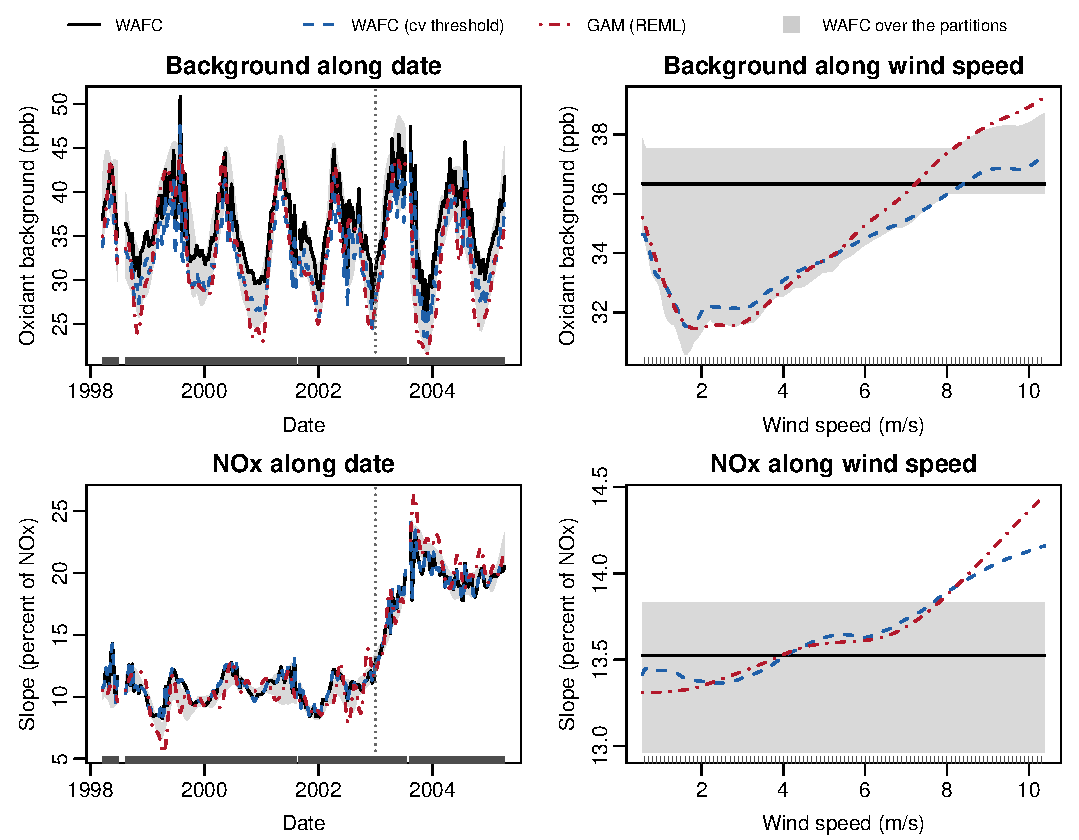
\includegraphics[width=\textwidth]{figures/marylebone.ukair.pdf}
\caption{Marylebone Road, London, hourly, 1998--2005: the oxidant background
(top, ppb) and the slope on NOx (bottom, percent of NOx) along the date
(left) and the wind speed (right), with the component of the other modulator
at its sample mean; the band is the range of the WAFC over 20 fits on 70\% of
the weeks. Not shown: the first and the last 60 days, where the periodized
basis joins the end of the series to its start, and the gaps in the data
longer than the spacing of the finest wavelets, about 11 days; ticks on the
axes mark the observed values.}
\label{fig:marylebone}
\end{figure}


\subsection{A second application}
\label{sec:app-beijing}

Section~S10 of the Supplementary Material applies the method to the hourly
PM2.5 at the site Dongsi in Beijing, from March 2013 to February 2017, in the
Beijing Multi-Site Air Quality data of the UCI Machine Learning Repository
\citep{Chen-UCI-2017, Zhang-Guo-Dong-He-Xu-Chen-2017}:
the logarithm of PM2.5 is regressed on the wind speed, the temperature and
the pressure, with coefficients modulated by the day of the year, a periodic
modulator, and the relative humidity, over 34,287 hours. The question there
is prediction. The coefficients change with the season, around the nominal
dates of the heating season, 15 November to 15 March
\citep[Section~7]{Liang-Zou-Guo-Li-Zhang-Zhang-Huang-Chen-2015}, and on the
held-out weeks the WAFC is ahead of the better of the two splines in all 20
partitions, with a root mean squared error 8\% below that of the better
spline on average.


%%%%%%%%%%%%%%%%%%%%%%%%%%%%%%%%%%%%%%%%%%%%%%%%%%%%%%%%%%%%%%%%%%%%%%%%%%%%%%
% E5b (k = 6): a Secao 7, com os numeros da E4.4 (results/tables/; o enquadramento
% combinado com o autor: o que o metodo entrega, onde nao ganha e por que, o que fica
% aberto).

